
%使用XeLaTeX编译
%版权所有,翻版必究
%本文件由程序自动生成,任何修改将被覆盖
%2019 年 01 月 23 日




%\FloatBarrier
\cleardoublepage
\chapter{
特效
}\label{c000015}






%使用XeLaTeX编译
%版权所有,翻版必究
%本文件由程序自动生成,任何修改将被覆盖
%2019 年 01 月 23 日





由于Qt Quick的所有渲染最终都
依靠现代3D可编程渲染管线实现。
这样用户就可以
在原有管线的基础上任意添加
新的渲染管线。

这样,读者可以不受限的将
所有现代渲染技术应用到
程序之中。

对于常见图形特效,Qt Quick
提供了“Qt Graphical Effects”
模块。

本章将带领读者纵览
Qt Graphical Effects提供的
25种图形特效。

\FloatBarrier
\section{
导引
}\label{c000015s000001}


%begin图片
\begin{figure}[htb] %浮动体 here and top ...
%there must use marginnote ...
\marginnote{\setlength\fboxsep{2pt}\fbox{\footnotesize{\kaishu\figurename\,}\footnotesize{\ref{p000012}}}}\centering %中心对齐
\includegraphics[width=0.95\textwidth]{../chapter06/firsteffect/the_app.png} %图片路径
\caption{文字阴影} %标题
\label{p000012} %索引
\end{figure}
%end图片



%使用XeLaTeX编译
%版权所有,翻版必究
%本文件由程序自动生成,任何修改将被覆盖
%2019 年 01 月 23 日



%begin表
\FloatBarrier                                  %强制完成浮动体布局
\begin{longtable}{cc}

%表头....
\toprule{}名称
&
描述[公式]%there must use marginnote ...
\marginnote{\setlength\fboxsep{2pt}\fbox{\footnotesize{\kaishu\tablename\,}\footnotesize{\ref{tb000002}}}}
\\ \midrule 
\endfirsthead

%表尾...
\bottomrule
\caption{混合类型}\label{tb000002} 
\endlastfoot

%重复表头
\toprule{}名称
&
描述[公式]
\\ \midrule
\endhead
%重复表尾
\midrule
\endfoot 
normal
    &
使用Alpha通道进行混合   
    \\

addition
    &
结果是source与foregroundSource的和
    \\

average
    &
结果是source与foregroundSource的均值
    \\

color
    &
结果是source的亮度值,
foregroundSource的色调与饱和度
    \\

colorBurn
    &
颜色加深$\left[v=1-(1-b)/a\right]$
 %与Photoshop colorBurn效果一致
    \\

colorDodge
    &
颜色减淡 $\left[v=b/(1-a)\right]$
 %与Photoshop colorDodge效果一致
    \\

darken
    &
变暗$\left[v=min(a,b)\right]$
 %与Photoshop  效果一致
    \\

darkerColor
    &
深色$\left[v=\begin{cases}
a, & a_r+a_r+a_b<b_r+b_g+b_b \\ 
b, & a_r+a_r+a_b>b_r+b_g+b_b
\end{cases}\right]$
 %与Photoshop  效果一致
    \\

difference
    &
    &
变暗$\left[v=abs(b-a)\right]$
 %与Photoshop  效果一致
    \\

divide
    &
    &
划分$\left[v=b/a\right]$
 %与Photoshop  效果一致
    \\

exclusion
    &
    &
排除$\left[v=b/a\right]$
 %与Photoshop  效果一致
    \\
\end{longtable}
%end表





%使用XeLaTeX编译
%版权所有,翻版必究
%本文件由程序自动生成,任何修改将被覆盖
%2019 年 01 月 23 日














%使用XeLaTeX编译
%版权所有,翻版必究
%本文件由程序自动生成,任何修改将被覆盖
%2019 年 01 月 23 日





%使用XeLaTeX编译
%版权所有,翻版必究
%本文件由程序自动生成,任何修改将被覆盖
%2019 年 01 月 23 日




\FloatBarrier
\section{
Blend
}\label{c000015s000002}


Blend特效常用属性
如\tablename\ \ref{tb000001}:


%使用XeLaTeX编译
%版权所有,翻版必究
%本文件由程序自动生成,任何修改将被覆盖
%2019 年 01 月 23 日



%begin表
\FloatBarrier                                  %强制完成浮动体布局
\begin{longtable}{cc}

%表头....
\toprule{}名称
&
描述[公式]%there must use marginnote ...
\marginnote{\setlength\fboxsep{2pt}\fbox{\footnotesize{\kaishu\tablename\,}\footnotesize{\ref{tb000002}}}}
\\ \midrule 
\endfirsthead

%表尾...
\bottomrule
\caption{混合类型}\label{tb000002} 
\endlastfoot

%重复表头
\toprule{}名称
&
描述[公式]
\\ \midrule
\endhead
%重复表尾
\midrule
\endfoot 
normal
    &
使用Alpha通道进行混合   
    \\

addition
    &
结果是source与foregroundSource的和
    \\

average
    &
结果是source与foregroundSource的均值
    \\

color
    &
结果是source的亮度值,
foregroundSource的色调与饱和度
    \\

colorBurn
    &
颜色加深$\left[v=1-(1-b)/a\right]$
 %与Photoshop colorBurn效果一致
    \\

colorDodge
    &
颜色减淡 $\left[v=b/(1-a)\right]$
 %与Photoshop colorDodge效果一致
    \\

darken
    &
变暗$\left[v=min(a,b)\right]$
 %与Photoshop  效果一致
    \\

darkerColor
    &
深色$\left[v=\begin{cases}
a, & a_r+a_r+a_b<b_r+b_g+b_b \\ 
b, & a_r+a_r+a_b>b_r+b_g+b_b
\end{cases}\right]$
 %与Photoshop  效果一致
    \\

difference
    &
    &
变暗$\left[v=abs(b-a)\right]$
 %与Photoshop  效果一致
    \\

divide
    &
    &
划分$\left[v=b/a\right]$
 %与Photoshop  效果一致
    \\

exclusion
    &
    &
排除$\left[v=b/a\right]$
 %与Photoshop  效果一致
    \\
\end{longtable}
%end表





%使用XeLaTeX编译
%版权所有,翻版必究
%本文件由程序自动生成,任何修改将被覆盖
%2019 年 01 月 23 日





混合类型
如\tablename\ \ref{tb000002}
    \footnote{$a$代表foregroundSource,
$b$代表source,
$0$代表黑色,
$1$代表白色,
$v$代表最终结果。}
:


%使用XeLaTeX编译
%版权所有,翻版必究
%本文件由程序自动生成,任何修改将被覆盖
%2019 年 01 月 23 日



%begin表
\FloatBarrier                                  %强制完成浮动体布局
\begin{longtable}{cc}

%表头....
\toprule{}名称
&
描述[公式]%there must use marginnote ...
\marginnote{\setlength\fboxsep{2pt}\fbox{\footnotesize{\kaishu\tablename\,}\footnotesize{\ref{tb000002}}}}
\\ \midrule 
\endfirsthead

%表尾...
\bottomrule
\caption{混合类型}\label{tb000002} 
\endlastfoot

%重复表头
\toprule{}名称
&
描述[公式]
\\ \midrule
\endhead
%重复表尾
\midrule
\endfoot 
normal
    &
使用Alpha通道进行混合   
    \\

addition
    &
结果是source与foregroundSource的和
    \\

average
    &
结果是source与foregroundSource的均值
    \\

color
    &
结果是source的亮度值,
foregroundSource的色调与饱和度
    \\

colorBurn
    &
颜色加深$\left[v=1-(1-b)/a\right]$
 %与Photoshop colorBurn效果一致
    \\

colorDodge
    &
颜色减淡 $\left[v=b/(1-a)\right]$
 %与Photoshop colorDodge效果一致
    \\

darken
    &
变暗$\left[v=min(a,b)\right]$
 %与Photoshop  效果一致
    \\

darkerColor
    &
深色$\left[v=\begin{cases}
a, & a_r+a_r+a_b<b_r+b_g+b_b \\ 
b, & a_r+a_r+a_b>b_r+b_g+b_b
\end{cases}\right]$
 %与Photoshop  效果一致
    \\

difference
    &
    &
变暗$\left[v=abs(b-a)\right]$
 %与Photoshop  效果一致
    \\

divide
    &
    &
划分$\left[v=b/a\right]$
 %与Photoshop  效果一致
    \\

exclusion
    &
    &
排除$\left[v=b/a\right]$
 %与Photoshop  效果一致
    \\
\end{longtable}
%end表





%使用XeLaTeX编译
%版权所有,翻版必究
%本文件由程序自动生成,任何修改将被覆盖
%2019 年 01 月 23 日





%begin图片
\begin{figure}[htb] %浮动体 here and top ...
%there must use marginnote ...
\marginnote{\setlength\fboxsep{2pt}\fbox{\footnotesize{\kaishu\figurename\,}\footnotesize{\ref{p000018}}}}\centering %中心对齐
\includegraphics[width=0.95\textwidth]{../chapter06/blend_effect/the_app.png} %图片路径
\caption{Blend} %标题
\label{p000018} %索引
\end{figure}
%end图片


%\begin{spacing}{1.0}
\refstepcounter{filesourcenumber}\label{f000052}    %增加源代码编号
\FloatBarrier                                  %强制完成浮动体布局
\begin{thebookfilesourceone}[escapeinside={(*@}{@*)},
caption=GoodLuck,
title=\filesourcenumbernameone \thefilesourcenumber
]
/*blend_effect/main.qml*/
import QtQuick 2.9
import QtGraphicalEffects 1.12

Rectangle {
    id : idRoot
    width: 640;
    height: 480;
    color: Qt.rgba(0.8,0.8,0.8,1);

    Image{
        anchors.fill: parent;
        source: "grass.jpg"
        fillMode: Image.Tile
        id : idGrass
        visible: false
    }

    Image{
        anchors.centerIn: parent;
        source: "bear.png"
        fillMode: Image.Stretch
        id : idBear
        visible: false
    }

    Blend{
        source: idGrass
        foregroundSource: idBear
        mode: idBlendControl.blendModeComboBox.currentText
        anchors.centerIn: parent;
        width: idBear.width
        height: idBear.height
    }

    BlendControl {
        id : idBlendControl
    }

}(*@\marginpar[\hfill\setlength\fboxsep{2pt}\fbox{\footnotesize{\kaishu\parbox{1em}{\setlength{\baselineskip}{2pt}\filesourcenumbernameone}}\footnotesize{\thefilesourcenumber}}]{\setlength\fboxsep{2pt}\fbox{\footnotesize{\kaishu\parbox{1em}{\setlength{\baselineskip}{2pt}\filesourcenumbernameone}}\footnotesize{\thefilesourcenumber}}}@*)\end{thebookfilesourceone}          %抄录环境
\addtocounter{lstlisting}{-1}   %sub lstlisting counter ...
%\end{spacing}


 






%使用XeLaTeX编译
%版权所有,翻版必究
%本文件由程序自动生成,任何修改将被覆盖
%2019 年 01 月 23 日





%使用XeLaTeX编译
%版权所有,翻版必究
%本文件由程序自动生成,任何修改将被覆盖
%2019 年 01 月 23 日





\begin{comment}
#version 150 core
in vec2 qt_TexCoord0;
uniform float qt_Opacity;
uniform sampler2D source;
uniform float brightness;
uniform float contrast;
out vec4 fragColor;

void main() {
    vec4 pixelColor = texture(source, qt_TexCoord0);
    pixelColor.rgb /= max(1.0/256.0, pixelColor.a);
    float c = 1.0 + contrast;
    float contrastGainFactor = 1.0 + c * c * c * c * step(0.0, contrast);
    pixelColor.rgb = ((pixelColor.rgb - 0.5) * (contrastGainFactor * contrast + 1.0)) + 0.5;
    pixelColor.rgb = mix(pixelColor.rgb, vec3(step(0.0, brightness)), abs(brightness));
    fragColor = vec4(pixelColor.rgb * pixelColor.a, pixelColor.a) * qt_Opacity;
}
\end{comment}


\FloatBarrier
\section{
BrightnessContrast
}\label{c000015s000003}


BrightnessContrast用于调整亮度和对比度。其常见属性
见\tablename\ \ref{tb000003}。


%使用XeLaTeX编译
%版权所有,翻版必究
%本文件由程序自动生成,任何修改将被覆盖
%2019 年 01 月 23 日



%begin表
\FloatBarrier                                  %强制完成浮动体布局
\begin{longtable}{cc}

%表头....
\toprule{}名称
&
描述[公式]%there must use marginnote ...
\marginnote{\setlength\fboxsep{2pt}\fbox{\footnotesize{\kaishu\tablename\,}\footnotesize{\ref{tb000002}}}}
\\ \midrule 
\endfirsthead

%表尾...
\bottomrule
\caption{混合类型}\label{tb000002} 
\endlastfoot

%重复表头
\toprule{}名称
&
描述[公式]
\\ \midrule
\endhead
%重复表尾
\midrule
\endfoot 
normal
    &
使用Alpha通道进行混合   
    \\

addition
    &
结果是source与foregroundSource的和
    \\

average
    &
结果是source与foregroundSource的均值
    \\

color
    &
结果是source的亮度值,
foregroundSource的色调与饱和度
    \\

colorBurn
    &
颜色加深$\left[v=1-(1-b)/a\right]$
 %与Photoshop colorBurn效果一致
    \\

colorDodge
    &
颜色减淡 $\left[v=b/(1-a)\right]$
 %与Photoshop colorDodge效果一致
    \\

darken
    &
变暗$\left[v=min(a,b)\right]$
 %与Photoshop  效果一致
    \\

darkerColor
    &
深色$\left[v=\begin{cases}
a, & a_r+a_r+a_b<b_r+b_g+b_b \\ 
b, & a_r+a_r+a_b>b_r+b_g+b_b
\end{cases}\right]$
 %与Photoshop  效果一致
    \\

difference
    &
    &
变暗$\left[v=abs(b-a)\right]$
 %与Photoshop  效果一致
    \\

divide
    &
    &
划分$\left[v=b/a\right]$
 %与Photoshop  效果一致
    \\

exclusion
    &
    &
排除$\left[v=b/a\right]$
 %与Photoshop  效果一致
    \\
\end{longtable}
%end表





%使用XeLaTeX编译
%版权所有,翻版必究
%本文件由程序自动生成,任何修改将被覆盖
%2019 年 01 月 23 日





BrightnessContrast的关键代码
见\filesourcenumbernameone\ \ref{f000077}。
%\begin{spacing}{1.0}
\refstepcounter{filesourcenumber}\label{f000077}    %增加源代码编号
\FloatBarrier                                  %强制完成浮动体布局
\begin{thebookfilesourceone}[escapeinside={(*@}{@*)},
caption=GoodLuck,
title=\filesourcenumbernameone \thefilesourcenumber
]
/*+glslcore/brightnesscontrast.frag*/
#version 150 core
in vec2 qt_TexCoord0;
uniform float qt_Opacity;
uniform sampler2D source;
uniform float brightness;
uniform float contrast;
out vec4 fragColor;

void main() {
    vec4 pixelColor = texture(source, qt_TexCoord0);
    pixelColor.rgb /= max(1.0/256.0, pixelColor.a);
    float c = 1.0 + contrast;
    float contrastGainFactor = 1.0 + c * c * c * c * step(0.0, contrast);
    pixelColor.rgb =
        ((pixelColor.rgb - 0.5) * (contrastGainFactor * contrast + 1.0)) + 0.5;
    pixelColor.rgb =
        mix(pixelColor.rgb, vec3(step(0.0, brightness)), abs(brightness));
    fragColor = vec4(pixelColor.rgb * pixelColor.a, pixelColor.a) * qt_Opacity;
}(*@\marginpar[\hfill\setlength\fboxsep{2pt}\fbox{\footnotesize{\kaishu\parbox{1em}{\setlength{\baselineskip}{2pt}\filesourcenumbernameone}}\footnotesize{\thefilesourcenumber}}]{\setlength\fboxsep{2pt}\fbox{\footnotesize{\kaishu\parbox{1em}{\setlength{\baselineskip}{2pt}\filesourcenumbernameone}}\footnotesize{\thefilesourcenumber}}}@*)\end{thebookfilesourceone}          %抄录环境
\addtocounter{lstlisting}{-1}   %sub lstlisting counter ...
%\end{spacing}


本节案例源码见\filesourcenumbernameone\ \ref{f000053}。

%begin图片
\begin{figure}[htb] %浮动体 here and top ...
%there must use marginnote ...
\marginnote{\setlength\fboxsep{2pt}\fbox{\footnotesize{\kaishu\figurename\,}\footnotesize{\ref{p000019}}}}\centering %中心对齐
\setlength\fboxsep{0pt}\fcolorbox[rgb]{0,0,0}{0.97,0.98,0.99}{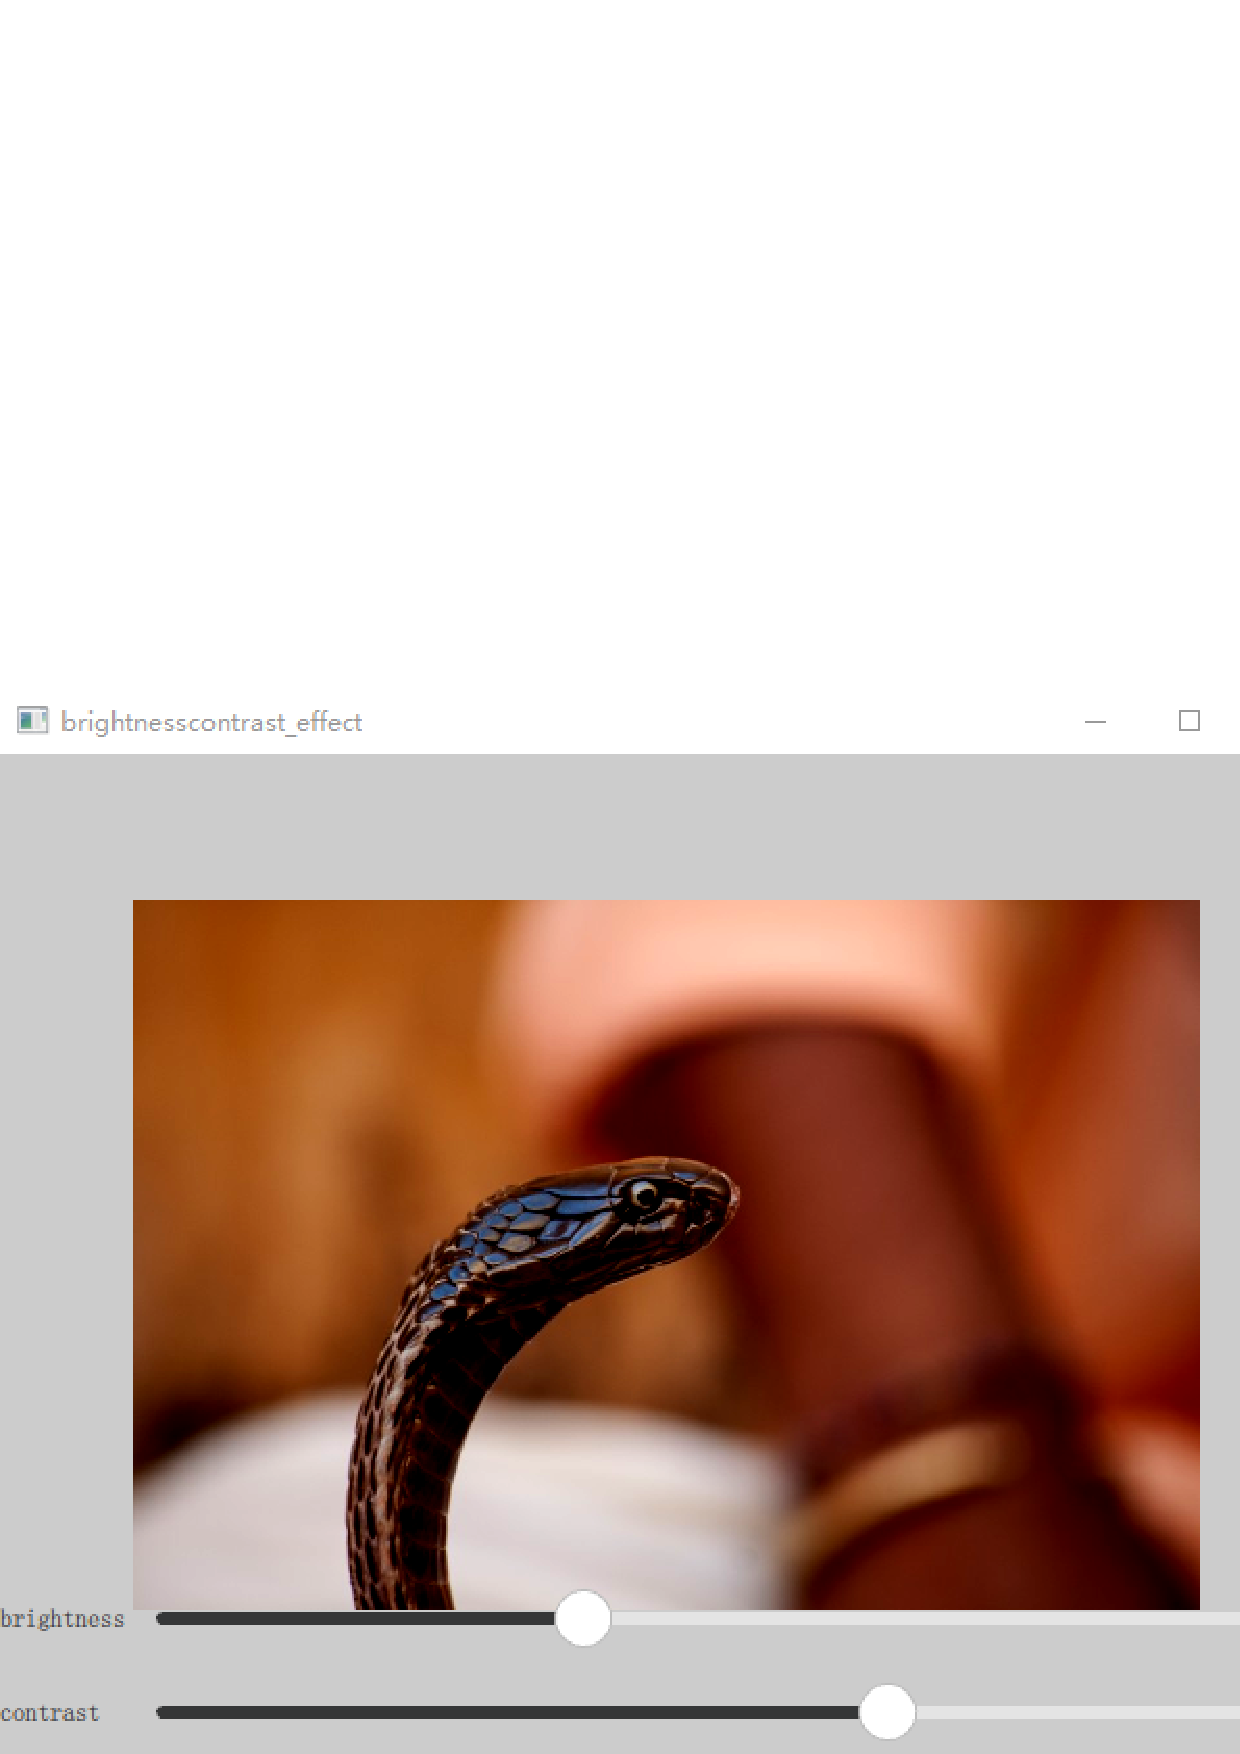
\includegraphics[width=0.95\textwidth]{the_book_image/p000019.pdf}} %图片路径
\caption{BrightnessContrast} %标题
\label{p000019} %索引
\end{figure}
%end图片


%\begin{spacing}{1.0}
\refstepcounter{filesourcenumber}\label{f000053}    %增加源代码编号
\FloatBarrier                                  %强制完成浮动体布局
\begin{thebookfilesourceone}[escapeinside={(*@}{@*)},
caption=GoodLuck,
title=\filesourcenumbernameone \thefilesourcenumber
]
/*brightnesscontrast_effect/main.qml*/
import QtQuick 2.9
import QtGraphicalEffects 1.12

Rectangle {

    id : idRoot
    width: 640;
    height: 480;
    color: Qt.rgba(0.8,0.8,0.8,1);


    Image{
        width: parent.width * 0.8;
        height: parent.height * 0.8;
        anchors.centerIn: parent
        source: "image.jpg"
        visible: false
        fillMode: Image.PreserveAspectFit
        id : idImage
    }

    BrightnessContrast{
        anchors.fill: idImage
        source: idImage
        contrast: idControl.contrastItem.value
        brightness: idControl.brightnessItem.value
    }

    BrightnessContrastControl{
        id:idControl
    }

}(*@\marginpar[\hfill\setlength\fboxsep{2pt}\fbox{\footnotesize{\kaishu\parbox{1em}{\setlength{\baselineskip}{2pt}\filesourcenumbernameone}}\footnotesize{\thefilesourcenumber}}]{\setlength\fboxsep{2pt}\fbox{\footnotesize{\kaishu\parbox{1em}{\setlength{\baselineskip}{2pt}\filesourcenumbernameone}}\footnotesize{\thefilesourcenumber}}}@*)\end{thebookfilesourceone}          %抄录环境
\addtocounter{lstlisting}{-1}   %sub lstlisting counter ...
%\end{spacing}



% ______all_key_words
% the_book_chapter the_book_subsection the_book_subsubsection
% the_book_section the_book_image the_book_table
% the_book_file the_book_tree_file the_book_command_file
% littlelongworld tabbing ref
% figurename tablename filesourcenumbernameone
% treeindexnumbernameone commandnumbernameone footnote
% item itemize comment textbullet
% \hspace*{\parindent}







%使用XeLaTeX编译
%版权所有,翻版必究
%本文件由程序自动生成,任何修改将被覆盖
%2019 年 01 月 23 日





%使用XeLaTeX编译
%版权所有,翻版必究
%本文件由程序自动生成,任何修改将被覆盖
%2019 年 01 月 23 日




\FloatBarrier
\section{
ColorOverlay
}\label{c000015s000004}



未完待续






%使用XeLaTeX编译
%版权所有,翻版必究
%本文件由程序自动生成,任何修改将被覆盖
%2019 年 01 月 23 日





%使用XeLaTeX编译
%版权所有,翻版必究
%本文件由程序自动生成,任何修改将被覆盖
%2019 年 01 月 23 日




\FloatBarrier
\section{
Colorize
}\label{c000015s000005}


%begin图片
\begin{figure}[htb] %浮动体 here and top ...
%there must use marginnote not use marginnote ...
\marginnote{\setlength\fboxsep{2pt}\fbox{\footnotesize{\kaishu\figurename\,}\footnotesize{\ref{p000021}}}}\centering %中心对齐
\includegraphics[width=0.95\textwidth]{../chapter06/colorize_effect/the_app.png} %图片路径
\caption{Colorize} %标题
\label{p000021} %索引
\end{figure}
%end图片


未完待续






%使用XeLaTeX编译
%版权所有,翻版必究
%本文件由程序自动生成,任何修改将被覆盖
%2019 年 01 月 23 日





%使用XeLaTeX编译
%版权所有,翻版必究
%本文件由程序自动生成,任何修改将被覆盖
%2019 年 01 月 23 日




\FloatBarrier
\section{
Desaturate
}\label{c000015s000006}


%begin图片
\begin{figure}[htb] %浮动体 here and top ...
%there must use marginnote not use marginnote ...
\marginnote{\setlength\fboxsep{2pt}\fbox{\footnotesize{\kaishu\figurename\,}\footnotesize{\ref{p000022}}}}\centering %中心对齐
\includegraphics[width=0.95\textwidth]{../chapter06/desaturate_effect/the_app.png} %图片路径
\caption{Desaturate} %标题
\label{p000022} %索引
\end{figure}
%end图片


未完待续






%使用XeLaTeX编译
%版权所有,翻版必究
%本文件由程序自动生成,任何修改将被覆盖
%2019 年 01 月 23 日




\input{chapter06/GammaAdjust.tex}

%使用XeLaTeX编译
%版权所有,翻版必究
%本文件由程序自动生成,任何修改将被覆盖
%2019 年 01 月 23 日




\FloatBarrier
\section{
HueSaturation
}\label{c000015s000008}


%begin图片
\begin{figure}[htb] %浮动体 here and top ...
%there must use marginnote ...
\marginnote{\setlength\fboxsep{2pt}\fbox{\footnotesize{\kaishu\figurename\,}\footnotesize{\ref{p000024}}}}\centering %中心对齐
\includegraphics[width=0.95\textwidth]{../chapter06/huesaturation_effect/the_app.png} %图片路径
\caption{HueSaturation} %标题
\label{p000024} %索引
\end{figure}
%end图片


%\begin{spacing}{1.0}
\refstepcounter{filesourcenumber}\label{f000058}    %增加源代码编号
\FloatBarrier                                  %强制完成浮动体布局
\begin{thebookfilesourceone}[escapeinside={(*@}{@*)},
caption=GoodLuck,
title=\filesourcenumbernameone \thefilesourcenumber
]
/*huesaturation_effect/main.qml*/
import QtQuick 2.9
import QtGraphicalEffects 1.12

Rectangle {
    id : idRoot
    width: 640;
    height: 480;
    color: Qt.rgba(0.8,0.8,0.8,1);

    Image{
        width: parent.width * 0.8;
        height: parent.height * 0.8;
        anchors.centerIn: parent
        source: "image"
        visible: false
        fillMode: Image.PreserveAspectFit
        id : idImage
    }

    HueSaturation{
        anchors.fill: idImage
        source: idImage
        hue : thisControl.hueItem.value
        lightness: thisControl.lightnessItem.value
        saturation: thisControl.saturationItem.value
    }

    HuesaturationControl{
        id : thisControl
    }

}(*@\marginpar[\hfill\setlength\fboxsep{2pt}\fbox{\footnotesize{\kaishu\parbox{1em}{\setlength{\baselineskip}{2pt}\filesourcenumbernameone}}\footnotesize{\thefilesourcenumber}}]{\setlength\fboxsep{2pt}\fbox{\footnotesize{\kaishu\parbox{1em}{\setlength{\baselineskip}{2pt}\filesourcenumbernameone}}\footnotesize{\thefilesourcenumber}}}@*)\end{thebookfilesourceone}          %抄录环境
\addtocounter{lstlisting}{-1}   %sub lstlisting counter ...
%\end{spacing}


未完待续






%使用XeLaTeX编译
%版权所有,翻版必究
%本文件由程序自动生成,任何修改将被覆盖
%2019 年 01 月 23 日




\input{chapter06/LevelAdjust.tex}
\input{chapter06/ConicalGradient.tex}
\input{chapter06/LinearGradient.tex}

%使用XeLaTeX编译
%版权所有,翻版必究
%本文件由程序自动生成,任何修改将被覆盖
%2019 年 01 月 23 日




\FloatBarrier
\section{
RadialGradient
}\label{c000015s000012}


%begin图片
\begin{figure}[htb] %浮动体 here and top ...
%there must use marginnote ...
\marginnote{\setlength\fboxsep{2pt}\fbox{\footnotesize{\kaishu\figurename\,}\footnotesize{\ref{p000028}}}}\centering %中心对齐
\setlength\fboxsep{0pt}\fcolorbox[rgb]{0,0,0}{0.97,0.98,0.99}{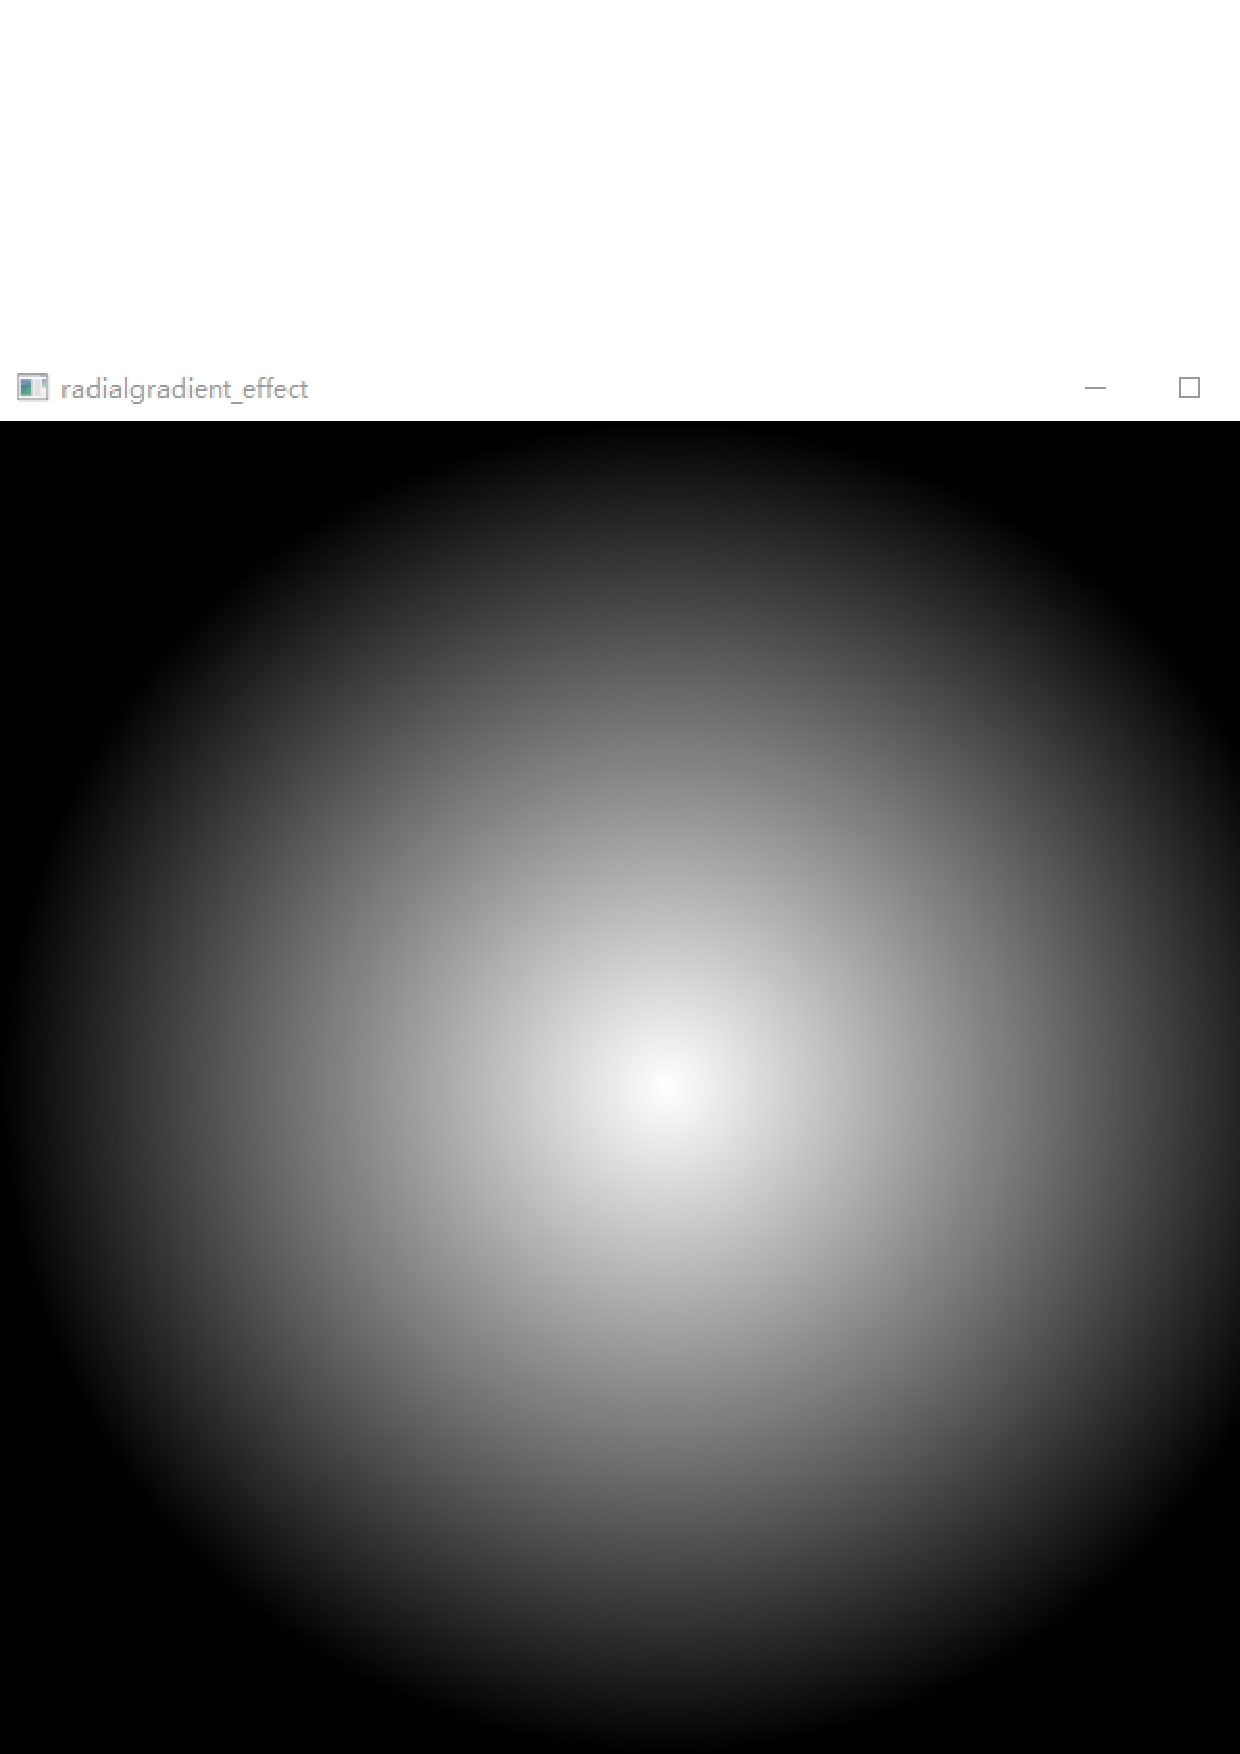
\includegraphics[width=0.95\textwidth]{the_book_image/p000028.pdf}} %图片路径
\caption{RadialGradient} %标题
\label{p000028} %索引
\end{figure}
%end图片


%\begin{spacing}{1.0}
\refstepcounter{filesourcenumber}\label{f000062}    %增加源代码编号
\FloatBarrier                                  %强制完成浮动体布局
\begin{thebookfilesourceone}[escapeinside={(*@}{@*)},
caption=GoodLuck,
title=\filesourcenumbernameone \thefilesourcenumber
]
/*radialgradient_effect/main.qml*/
import QtQuick 2.9
import QtGraphicalEffects 1.12

Rectangle {
    id : idRoot
    width: 640;
    height: 640;
    color: Qt.rgba(0.8,0.8,0.8,1);

    RadialGradient {
        anchors.fill: parent
        gradient: Gradient {
            GradientStop { position: 0.0; color: "white" }
            GradientStop { position: 0.5; color: "black" }
        }
    }

}(*@\marginpar[\hfill\setlength\fboxsep{2pt}\fbox{\footnotesize{\kaishu\parbox{1em}{\setlength{\baselineskip}{2pt}\filesourcenumbernameone}}\footnotesize{\thefilesourcenumber}}]{\setlength\fboxsep{2pt}\fbox{\footnotesize{\kaishu\parbox{1em}{\setlength{\baselineskip}{2pt}\filesourcenumbernameone}}\footnotesize{\thefilesourcenumber}}}@*)\end{thebookfilesourceone}          %抄录环境
\addtocounter{lstlisting}{-1}   %sub lstlisting counter ...
%\end{spacing}


未完待续


% ______all_key_words
% the_book_chapter the_book_subsection the_book_subsubsection
% the_book_section the_book_image the_book_table
% the_book_file the_book_tree_file the_book_command_file
% littlelongworld tabbing ref
% figurename tablename filesourcenumbernameone
% treeindexnumbernameone commandnumbernameone footnote 
% item itemize comment textbullet
% \hspace*{\parindent}







%使用XeLaTeX编译
%版权所有,翻版必究
%本文件由程序自动生成,任何修改将被覆盖
%2019 年 01 月 23 日





%使用XeLaTeX编译
%版权所有,翻版必究
%本文件由程序自动生成,任何修改将被覆盖
%2019 年 01 月 23 日




\FloatBarrier
\section{
Displace
}\label{c000015s000013}


%begin图片
\begin{figure}[htb] %浮动体 here and top ...
%there must use marginnote not use marginnote ...
\marginnote{\setlength\fboxsep{2pt}\fbox{\footnotesize{\kaishu\figurename\,}\footnotesize{\ref{p000029}}}}\centering %中心对齐
\includegraphics[width=0.95\textwidth]{../chapter06/displace_effect/the_app.png} %图片路径
\caption{Displace} %标题
\label{p000029} %索引
\end{figure}
%end图片


未完待续






%使用XeLaTeX编译
%版权所有,翻版必究
%本文件由程序自动生成,任何修改将被覆盖
%2019 年 01 月 23 日




\input{chapter06/DropShadow.tex}
\input{chapter06/InnerShadow.tex}
\input{chapter06/FastBlur.tex}

%使用XeLaTeX编译
%版权所有,翻版必究
%本文件由程序自动生成,任何修改将被覆盖
%2019 年 01 月 23 日




\FloatBarrier
\section{
GaussianBlur
}\label{c000015s000017}


%begin图片
\begin{figure}[htb] %浮动体 here and top ...
%there must use marginnote not use marginnote ...
\marginnote{\setlength\fboxsep{2pt}\fbox{\footnotesize{\kaishu\figurename\,}\footnotesize{\ref{p000033}}}}\centering %中心对齐
\includegraphics[width=0.95\textwidth]{../chapter06/gaussianblur_effect/the_app.png} %图片路径
\caption{GaussianBlur} %标题
\label{p000033} %索引
\end{figure}
%end图片


%\begin{spacing}{1.0}
\refstepcounter{filesourcenumber}\label{f000067}    %增加源代码编号
\FloatBarrier                                  %强制完成浮动体布局
\begin{thebookfilesourceone}[escapeinside={(*@}{@*)},
caption=GoodLuck,
title=\filesourcenumbernameone \thefilesourcenumber
]
/*gaussianblur_effect/main.qml*/
import QtQuick 2.9
import QtGraphicalEffects 1.12

Rectangle {
    id : idRoot
    width: 640;
    height: 480;
    color: Qt.rgba(0.8,0.8,0.8,1);

    Image{
        width: parent.width * 0.8;
        height: parent.height * 0.8;
        anchors.centerIn: parent
        source: "image"
        visible: false
        fillMode: Image.PreserveAspectFit
        id : idImage
    }

    GaussianBlur{
        anchors.fill: idImage
        source: idImage
        radius: 8
        samples: 16
        deviation: idThisControl.deviationItem.value
    }

    GaussianBlurControl{
        id : idThisControl
    }

}(*@\marginpar[\hfill\setlength\fboxsep{2pt}\fbox{\footnotesize{\kaishu\parbox{1em}{\setlength{\baselineskip}{2pt}\filesourcenumbernameone}}\footnotesize{\thefilesourcenumber}}]{\setlength\fboxsep{2pt}\fbox{\footnotesize{\kaishu\parbox{1em}{\setlength{\baselineskip}{2pt}\filesourcenumbernameone}}\footnotesize{\thefilesourcenumber}}}@*)\end{thebookfilesourceone}          %抄录环境
\addtocounter{lstlisting}{-1}   %sub lstlisting counter ...
%\end{spacing}


未完待续






%使用XeLaTeX编译
%版权所有,翻版必究
%本文件由程序自动生成,任何修改将被覆盖
%2019 年 01 月 23 日




\input{chapter06/MaskedBlur.tex}
\input{chapter06/RecursiveBlur.tex}

%使用XeLaTeX编译
%版权所有,翻版必究
%本文件由程序自动生成,任何修改将被覆盖
%2019 年 01 月 23 日




\FloatBarrier
\section{
DirectionalBlur
}\label{c000015s000020}


%begin图片
\begin{figure}[htb] %浮动体 here and top ...
%there must use marginnote ...
\marginnote{\setlength\fboxsep{2pt}\fbox{\footnotesize{\kaishu\figurename\,}\footnotesize{\ref{p000036}}}}\centering %中心对齐
\setlength\fboxsep{0pt}\fcolorbox[rgb]{0,0,0}{0,0,0}{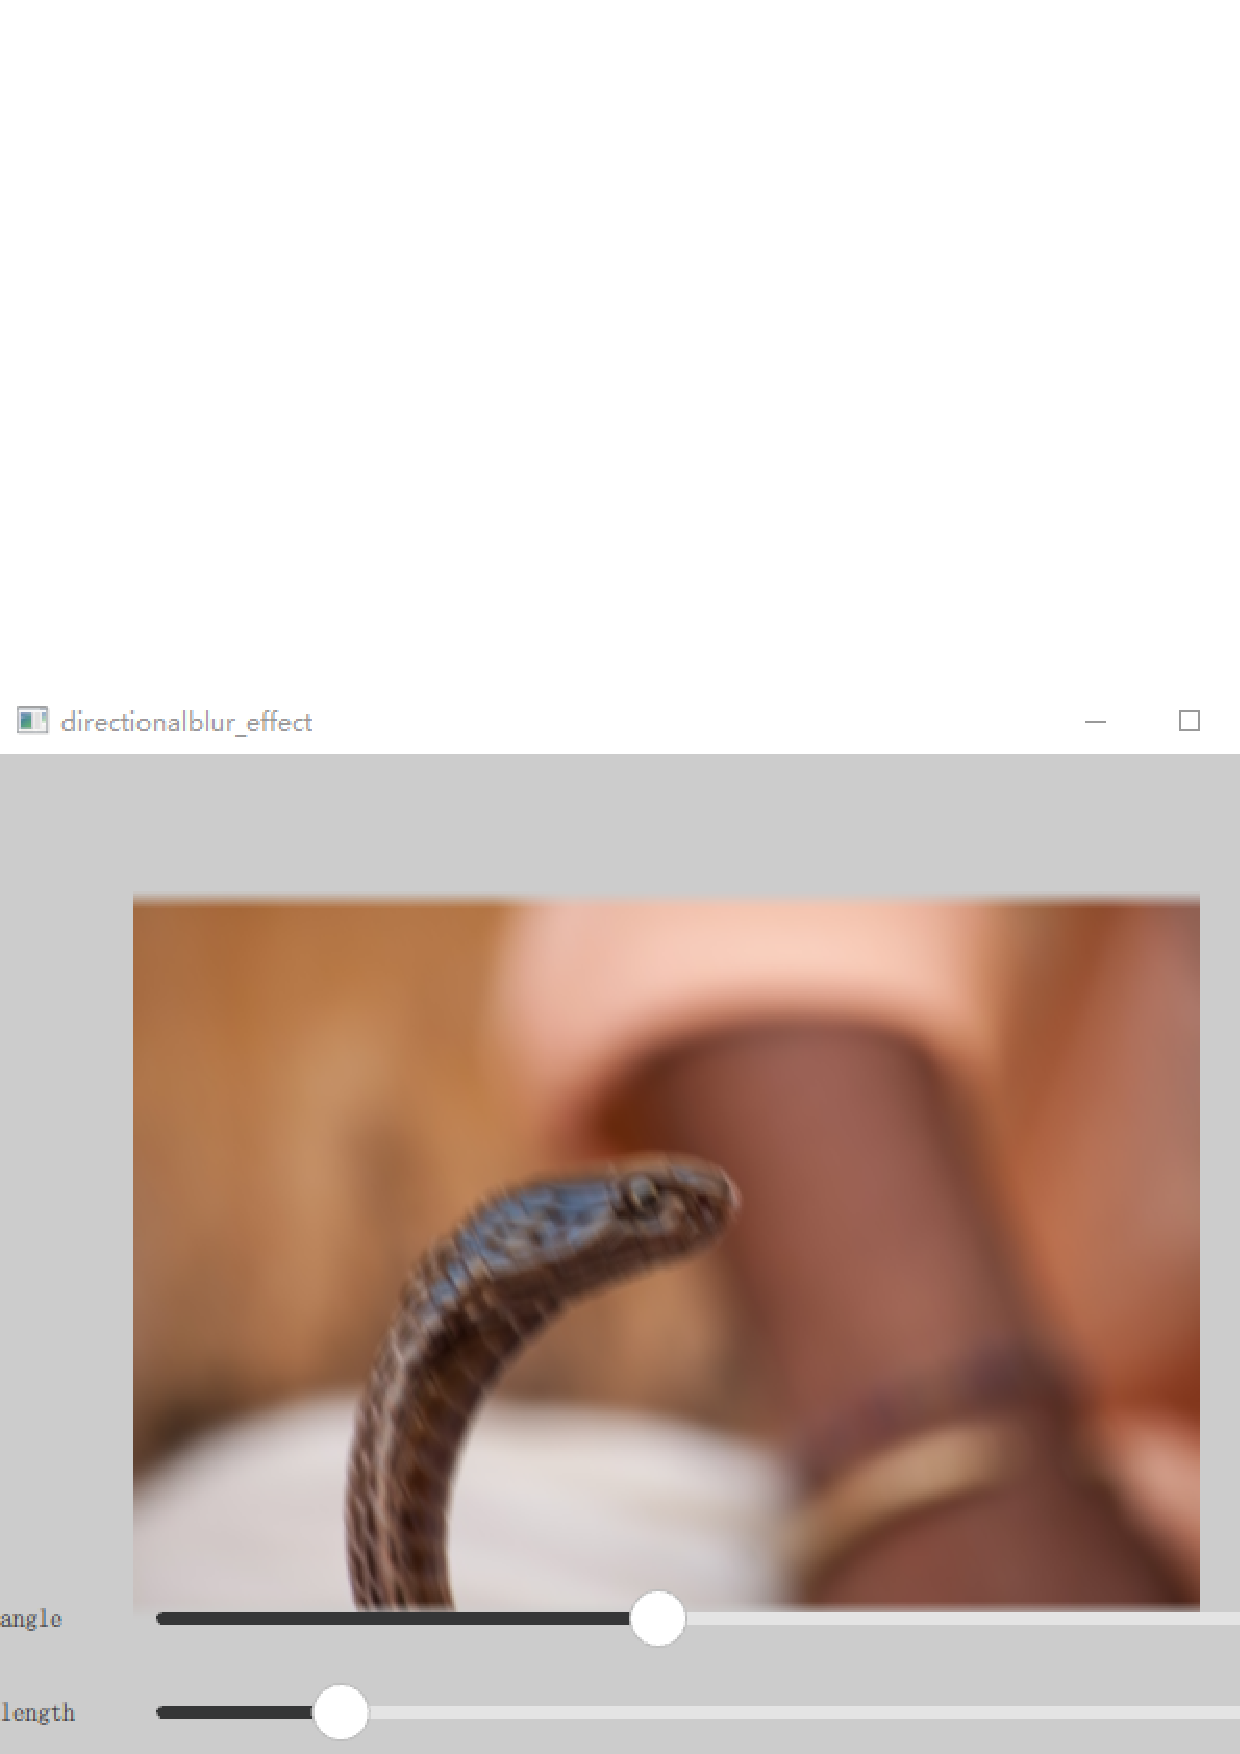
\includegraphics[width=0.95\textwidth]{the_book_image/p000036.pdf}} %图片路径
\caption{DirectionalBlur} %标题
\label{p000036} %索引
\end{figure}
%end图片


%\begin{spacing}{1.0}
\refstepcounter{filesourcenumber}\label{f000070}    %增加源代码编号
\FloatBarrier                                  %强制完成浮动体布局
\begin{thebookfilesourceone}[escapeinside={(*@}{@*)},
caption=GoodLuck,
title=\filesourcenumbernameone \thefilesourcenumber
]
/*directionalblur_effect/main.qml*/
import QtQuick 2.9
import QtGraphicalEffects 1.12

Rectangle {
    id : idRoot
    width: 640;
    height: 480;
    color: Qt.rgba(0.8,0.8,0.8,1);

    Image{
        width: parent.width * 0.8;
        height: parent.height * 0.8;
        anchors.centerIn: parent
        source: "image.jpg"
        visible: false
        fillMode: Image.PreserveAspectFit
        id : idImage
    }

    DirectionalBlur{
        anchors.fill: idImage
        source: idImage
        samples: 64
        length: idThisControl.lengthItem.value
        angle: idThisControl.angleItem.value
        transparentBorder : false
        id:idEffect
    }

    DirectionalblurControl{
        id : idThisControl
        lengthItem.to: idEffect.samples
    }

}(*@\marginpar[\hfill\setlength\fboxsep{2pt}\fbox{\footnotesize{\kaishu\parbox{1em}{\setlength{\baselineskip}{2pt}\filesourcenumbernameone}}\footnotesize{\thefilesourcenumber}}]{\setlength\fboxsep{2pt}\fbox{\footnotesize{\kaishu\parbox{1em}{\setlength{\baselineskip}{2pt}\filesourcenumbernameone}}\footnotesize{\thefilesourcenumber}}}@*)\end{thebookfilesourceone}          %抄录环境
\addtocounter{lstlisting}{-1}   %sub lstlisting counter ...
%\end{spacing}


未完待续






%使用XeLaTeX编译
%版权所有,翻版必究
%本文件由程序自动生成,任何修改将被覆盖
%2019 年 01 月 23 日




\input{chapter06/RadialBlur.tex}

%使用XeLaTeX编译
%版权所有,翻版必究
%本文件由程序自动生成,任何修改将被覆盖
%2019 年 01 月 23 日




\FloatBarrier
\section{
ZoomBlur
}\label{c000015s000022}


%begin图片
\begin{figure}[htb] %浮动体 here and top ...
%there must use marginnote not use marginnote ...
\marginnote{\setlength\fboxsep{2pt}\fbox{\footnotesize{\kaishu\figurename\,}\footnotesize{\ref{p000038}}}}\centering %中心对齐
\includegraphics[width=0.95\textwidth]{../chapter06/zoomblur_effect/the_app.png} %图片路径
\caption{ZoomBlur} %标题
\label{p000038} %索引
\end{figure}
%end图片


未完待续






%使用XeLaTeX编译
%版权所有,翻版必究
%本文件由程序自动生成,任何修改将被覆盖
%2019 年 01 月 23 日




\input{chapter06/Glow.tex}

%使用XeLaTeX编译
%版权所有,翻版必究
%本文件由程序自动生成,任何修改将被覆盖
%2019 年 01 月 23 日




\FloatBarrier
\section{
RectangularGlow
}\label{c000015s000024}


%begin图片
\begin{figure}[htb] %浮动体 here and top ...
%there must use marginnote not use marginnote ...
\marginnote{\setlength\fboxsep{2pt}\fbox{\footnotesize{\kaishu\figurename\,}\footnotesize{\ref{p000040}}}}\centering %中心对齐
\includegraphics[width=0.95\textwidth]{../chapter06/rectangularglow_effect/the_app.png} %图片路径
\caption{RectangularGlow} %标题
\label{p000040} %索引
\end{figure}
%end图片


未完待续






%使用XeLaTeX编译
%版权所有,翻版必究
%本文件由程序自动生成,任何修改将被覆盖
%2019 年 01 月 23 日




\input{chapter06/OpacityMask.tex}
\input{chapter06/ThresholdMask.tex}




% ______all_key_words
% the_book_chapter the_book_subsection the_book_subsubsection
% the_book_section the_book_image the_book_table
% the_book_file the_book_tree_file the_book_command_file
% littlelongworld tabbing ref
% figurename tablename filesourcenumbernameone
% treeindexnumbernameone commandnumbernameone footnote 
% item itemize comment textbullet
% \hspace*{\parindent}







%使用XeLaTeX编译
%版权所有,翻版必究
%本文件由程序自动生成,任何修改将被覆盖
%2019 年 01 月 23 日



